\chapter{Estudo de Caso: Noosfero}
\label{noosfero}
%------------------------------------------------------------------------------%
Durante o quarto capítulo deste trabalho de conclusão de curso, discutiremos sobre 
o ambiente de trabalho e a plataforma de desenvolvimento, chamada Noosfero, assim 
como os testes e as funcionalidades desenvolvidas dentro do processo de colaboração 
com esta plataforma.
%
Noosfero\footnote{\url{noosfero.org}} é uma plataforma desenvolvida pela Colivre (Cooperativa de Tecnologias
Livre)\footnote{url{colivre.coop.br}}, possui licença AGPL e é utilizado, principalmente em universidades públicas,
para desenvolvimento de redes colaborativas. \footnote{url{http://softwarelivre.org/colivre/blog/projeto-noosfero}}
%
O noosfero foi desenvolvido na linguagem de programação Ruby, versão 1.8.7, e utiliza
o framework Model-View-Controller (MVC) para aplicações web Ruby on Rails, versão 
2.3.5. A escolha destas tecnologias, por parte dos criadores do Noosfero foi baseada 
fato de que o Ruby possui sintaxe simples, elegante e de fácil leitura, o que aumenta
a manutenibilidade do sistema, uma característica importante num projeto de software
livre que visa atrair desenvolvedores externos~\cite{meirelles2013}.

%------------------------------------------------------------------------------%
\section{Desenvolvimento no processo de colaboração ao noosfero}
Por tratar de um software livre, a plataforma Noosfero possui uma grande quantidade 
de colaboradores, formado por equipes de desenvolvimento como na Universidade de 
Brasília, ou por desenvolvedores independentes. Assim, para que haja sucesso na 
colaboração, são feitas exigências durante o desenvolvimento, assim como testes 
bem definidos para aprovar novas funcionalidade.%Referenciar%
%
De acordo com os contribuidores do noosfero, a plataforma livre possui as seguintes 
caracteristicas:
%
\begin{enumerate}
\item Rede Social (três entidades: pessoas, comunidades e organizações); 
\item  CMS: pastas, artigos, RSS, upload e publicação de imagens e arquivos; 
\item  \textit{Blog} com sistema de notificação de comentários; 
\item  Galeria de imagens; 
\item  e-Portfolios (individuais e de grupos); 
\item  Compartilhar interesses; 
\item  Fóruns / Discussão temática; 
\item  Agenda de eventos compartilhadas; 
\item  Vitrine digital para exposição de produtos e serviços e carrinho de compras; 
\item  Acompanhamento de atividades de usuários e grupos; 
\item  Mensagens assíncronas e \textit{web chat}. 
\end{enumerate}
%
Além da utilização da linguagem de programação \textit{Ruby}, o desenvolvimento da plataforma 
noosfero também se baseia em JavaScript, CSS, dentre outras linguagens, como pode-se 
ver na figura abaixo:
%
\begin{figure}[!h]
    \centering
    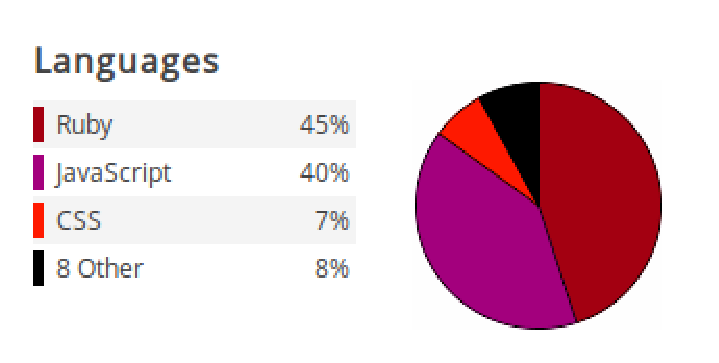
\includegraphics[keepaspectratio=true,scale=0.60]
      {figuras/noosfero.eps}
    \caption{Desenvolvimento noosfero \footnote{url{noosfero.org}}}
    \label{noosfero}
\end{figure}

%------------------------------------------------------------------------------%
\subsection{Ciclo de desenvolvimento do noosfero}
%
O desenvolvimento para a plataforma Noosfero é realizado em ciclos e, pela Colivre, 
possui as seguintes fases: desenvolvimento, release 1, release 2 e release final.
%
\subsubsection{Fase de Desenvolvimento}
%
Antes da fase de desenvolvimento for iniciada é necessário que seja feita a 
documentação do que será desenvolvido. Os desenvolvedores responsáveis criam um 
\textit{action item} (item de ação), contendo a história de usuário ou os requisitos do novo 
recurso. Um \textit{action item} pode ser descrito como uma \textit{feature} (novo recurso) ou como 
um \textit{bug} (defeito) encontrado, como demonstrado nas figuras abaixo:\footnote{url{noosfero.org}}
%
\begin{figure}[!h]
    \centering
    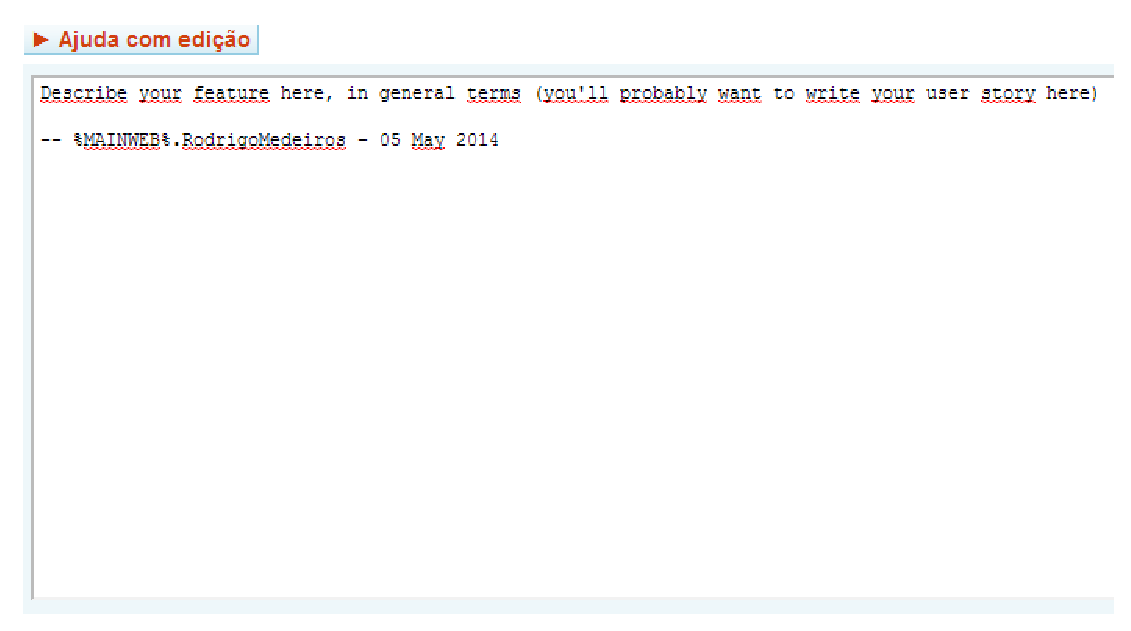
\includegraphics[keepaspectratio=true,scale=0.65]
      {figuras/noosfero_feature.eps}
    \caption{Descrição de \textit{feature} - noosfero}
    \label{noosfero_feature}
\end{figure}
%
\begin{figure}[!h]
    \centering
    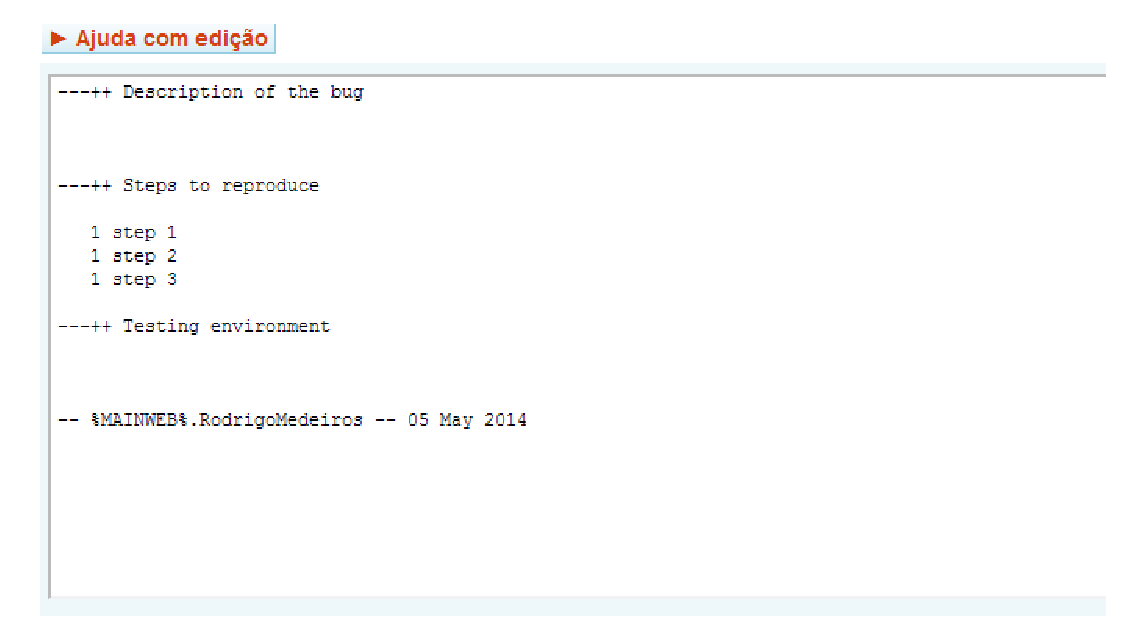
\includegraphics[keepaspectratio=true,scale=0.65]
      {figuras/noosfero_bug.eps}
    \caption{Descrição de \textit{bug} - noosfero}
    \label{noosfero_bug}
\end{figure}

%------------------------------------------------------------------------------%

Além da documentação, é necessário o envio de um \textit{email} a comunidade descrevendo o 
que será desenvolvido. A partir deste \textit{email}, a comunidade irá avaliar a funcionalidade 
descrita e decidir se é um funcionalidade importante para se incorporar ou não. 
Este processo de avaliação tem a duração de uma semana, geralmente.\footnote{url{noosfero.org}}

Com a aprovação da comunidade são feitas as revisões do ciclo de desenvolvimento, 
que deve seguir os seguintes passos:
%
\begin{enumerate}
\item Criar um \textit{‘merge request’} juntamente com o código;
\item Código é revisado pela comunidade;
\item Código é bom? 
\subitem Se sim:
\subsubitem Vá para o passo 4;
\subitem Se não:
\subsubitem \textit{‘Merge request’} é rejeitado e as razões por tal são comentadas e 
respondidas;
\subsubitem Desenvolvedores revisam o que está errado;
\item Código é incluido no código principal.
\end{enumerate}
%------------------------------------------------------------------------------%
\subsubsection{Fase de Release 1}
%
A entrega da \textit{release} consiste na instalação da nova versão do código no repositório 
de testes, assim como no código principal quando não houver mais defeitos, ou todos 
os defeitos encontrados forem tratados devidamente. Porém se algum erro crítico for 
encontrado e não for tratado a tempo da \textit{release} final, o lançamento pode ser adiado 
para a próxima \textit{release}.
%
\subsubsection{Fase de Release 2}
%
A \textit{release} 2 não é obrigatória, so ocorre se houver muitas mudanças na \textit{release} 1 e 
requerer novos testes. Vale lembrar que os procedimentos realizados para aprovar a 
\textit{release} 2 são os mesmos da \textit{release} 1%Referenciar%
%
\subsubsection{Release Final}
%
A versão final do código é lançada após todos os testes serem aprovados nas \textit{releases} 
1 e 2, assim o código pode ser atualizado para o código principal do noosfero, 
encerrando o ciclo de desenvolvimento.\footnote{url{noosfero.org}}

%------------------------------------------------------------------------------%

\section{Testes no processo de colaboração ao noosfero}
%
Os responsáveis por manter o noosfero, pessoas que aprovam as solicitações de 
alteração na plataforma, exigem que os \textit{plugins} passem por uma bateria de testes 
para que esses \textit{plugins} tenham capacidade de ser incorporados à uma versão do 
noosfero, prevenindo assim uma possível  inserção de código defeituoso que possa 
afetar o núcleo da plataforma até outros  \textit{plugins}, além de manter a qualidade de 
código no padrão desejado.
%
Alguns testes automatizados são realizados no noosfero para validação de novos 
recursos de software, dentre eles estão: testes funcionais, testes de aceitação e 
testes unitários, testes estes que são executados na própria plataforma do noosfero.
%
\subsection{Testes de aceitação - Cucumber}
Os testes de aceitação, que possuem uma visão mais voltada para o usuário, fazem 
parte de uma fase do processo de teste em que um teste de caixa-preta é realizado 
num sistema antes de sua disponibilização. Para isso utilizamos o cucumber, uma 
ferramenta que pode executar documentação de funcionalidades escrita em texto puro. 
Com base nesta especificações, o cucumber executa testes.
%
O cucumber proporciona uma melhor comunicação entre equipe de desenvolvimento e 
cliente, por utilizar uma linguagem  em texto puro.
%
No cucumber, uma \textit{feature} é um requisito de alto nível 
expressado da pespectiva de uma pessoa e possui uma estrutura similar as histórias 
de usuário do XP~\citeonline{chelimsky2010}. Essa estrutura é proposta da seguinte forma:
\begin{enumerate}
\item \textbf{Título:} Palavra-chave ‘\textit{feature}’ e um título curto que representa o 
objetivo da \textit{feature}.
\item \textbf{Narrativa:} um texto curto que demonstre os cenários de execução, 
exatamente como a narrativa de uma história de usuário:

\begin{figure}[!h]
    \centering
    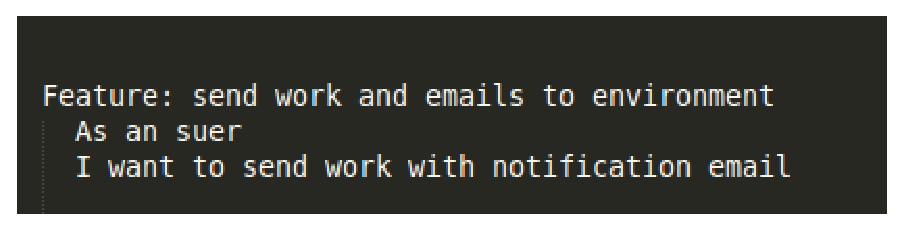
\includegraphics[keepaspectratio=true,scale=0.50]
      {figuras/noosfero_feature2.eps}
    \caption{Descrição do título (\textit{feature}) de um teste}
    \label{nosfero_feature}
\end{figure}

\item \textbf{Pré condições:} representado pela palavra-chave \textit{'background'}, define os passos 
precedem cada cenário de teste.

\begin{figure}[!h]
    \centering
    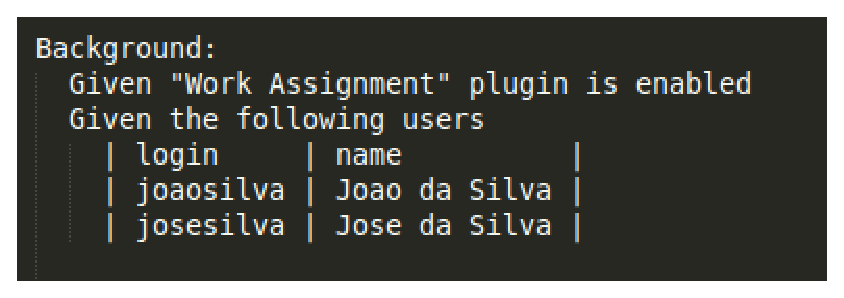
\includegraphics[keepaspectratio=true,scale=0.50]
      {figuras/noosfero_back.eps}
    \caption{Descrição de pré condições (\textit{background}) de um teste}
    \label{nosfero_feature}
\end{figure}

\item \textbf{Cenários:} representam parte concreta de como o software deve se 
comportar, e sendo a parte essencial do teste realizado no 
cucumber. Após a palavra-chave \textit{‘scenario’} define-se o nome do cenário em questão:
\item \textbf{Passos:} Cada cenario possui uma série de passos que demontram o seu 
comportamento, que são linhas simples iniciadas com as seguintes palavras-chaves: 
\textit{Given, When, Then, And, But}.
\item \textbf{Given:} Indica uma condição inicial para que o cenário seja executado, 
trata-se das pré-condições do cenário.
\item \textbf{When:} Indica o evento do cenário
\item \textbf{Then:} Indica o que é esperado após o evento ocorrer.

\begin{figure}[!h]
    \centering
    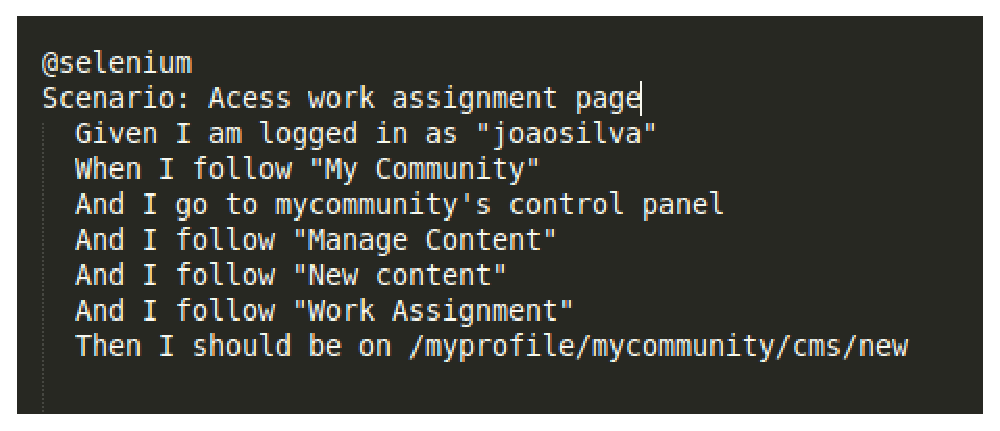
\includegraphics[keepaspectratio=true,scale=0.50]
      {figuras/noosfero_scenario.eps}
    \caption{Descrição do cenário (\textit{scenario}) de um teste}
    \label{nosfero_scenario}
\end{figure}

\end{enumerate}
Além do cucumber, também é utilizado um software chamado selenium, que é uma ferramenta
usada para desenvolver casos de testes a partir de \textit{web browsers}, como o mozilla firefox. 
Estas duas ferramentas, cucumber e selenium, utilizadas em conjunto, proporciona ao desenvolvedor
a facilidade ao escrever os casos de testes em linguagem pura simular a execução automática
destes testes em um \textit{web browser}.
%
Porém o cucumber não faz tudo em linguagem pura, é necessário que outro código seja desenvolvido,
em Ruby, fazendo par por baixo dos panos com a linguagem pura e executando os testes~\cite{akita2011}.


%------------------------------------------------------------------------------%
\subsection{Testes Funcionais e Unitários}
%
Os testes funcionais tem como objetivo no desenvolvimento na plataforma noosfero, verificar
a integraçao da aplicação desenvolvida.
%
Os testes unitários são executados em conjunto com os testes funcionais, porém  com o objetivo
de verificar trechos menores de códigos.
%
Assim os testes funcionais e unitários são escritos da seguinte forma:

\textbf{Setup:} indica as condições inciais dos testes, setando variáveis de ambiente e de 
configuração por exemplo.

\begin{figure}[!h]
    \centering
    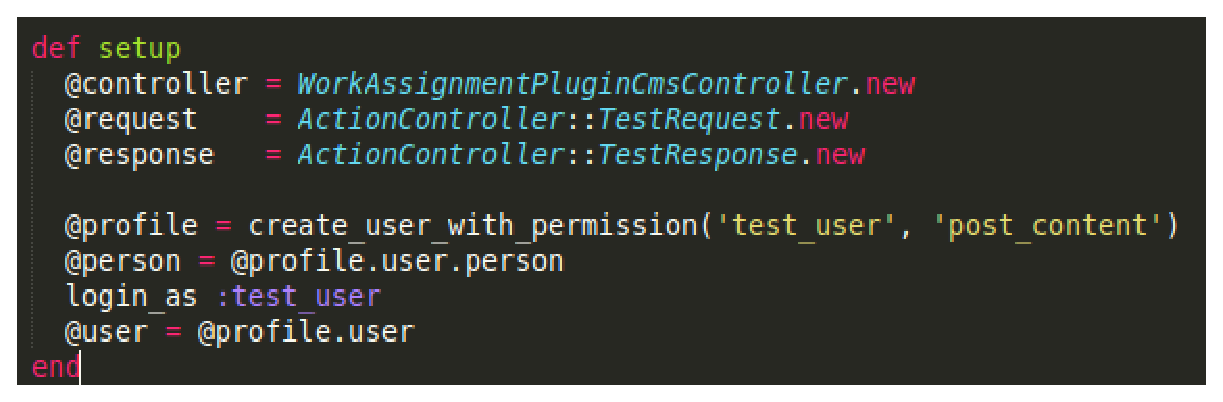
\includegraphics[keepaspectratio=true,scale=0.5]
      {figuras/teste_setup.eps}
    \caption{Descrição do setup de um teste}
    \label{nosfero_setup}
\end{figure}

\textbf{Título:} título do teste iniciado com a palavra \textit{‘should’} e finalizado com \textit{‘do’}

\textbf{Passos:} código que define o comportamento do teste

\textbf{Verificação:} Assertiva que verifica se a ação foi realizada como esperada.

\begin{figure}[!h]
    \centering
    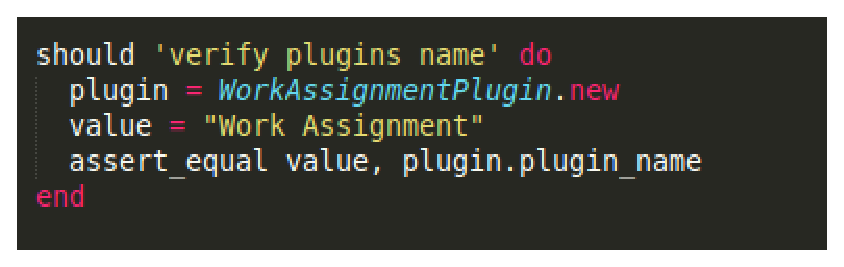
\includegraphics[keepaspectratio=true,scale=0.55]
      {figuras/teste_should.eps}
    \caption{Código de teste}
    \label{noosfero_should}
\end{figure}

%------------------------------------------------------------------------------%

\section{Funcionalidades desenvolvidas}

O processo de desenvolvimento de software, assim como o desenvolvimento de testes 
deste trabalho de conclusão de curso teve seu enfoque na rede colaborativa baseada 
no noosfero desenvolvida para a Universidade de Brasília (UnB)\footnote{\url{www.unb.br}},
trata-se na rede chamada de Comunidade UnB, que se encontra em ambiente de testes, 
porém disponível para acesso externo, contando com aproximadamente 160 usuários ativos. A rede 
Comunidade UnB é uma instância do noosfero instalada através de um pacote em um 
servidor do Centro de Difusão de Tecnologia e Conhecimetno (CDTC)\footnote{\url{www.cdtc.org.br}} da UnB.
%
O propósito da rede Comunidade UnB é tornar-se um ambiente de colaboração entre os 
alunos da Universidade de Brasília, tanto de graduação quanto de pós-graduação, 
possibilitando criação comunidades e blogs para discussões, ou a disponibilização 
de artigos, trabalhos de graduação e pós-graduação onde qualquer membro da universidade 
tenha acesso.
%
Para que este propósito seja cumprido, funcionalidades importantes do Comunidade 
UnB precisavam ser desenvolvidas. Ao decorrer deste trabalho de graduação, foram 
desenvolvidos, juntamente com seus respectivos testes, alguns plugins que serão 
descritos abaixo.
%------------------------------------------------------------------------------%
\subsection{Plugin Ldap UnB}
%
Como rede colaborativa dos membros da Universidade de Brasília, o Comunidade UnB 
necessita possuir restrição de acesso aos usuários, para que somente membros ativos 
da universidade tenham acesso ao conteúdo da rede colaborativa. 
%
Para que esta necessidade fosse satisfeita foi desenvolvido um \textit{plugin} no noosfero, 
que efetuasse as restrições necessárias, utilizando o protocolo de autenticação da 
UnB, o LDAP.
%
\textit{Lightweight Directory Access Protocol} (LDAP) é um protocolo de aplicação 
aberto para acesso e manutenção  de serviços de informação de diretório distribuídos 
na internet~\cite{sermersheim2006}.
%
Os serviços de diretório desempenham um papel importante no desenvolvimento de aplicativos 
de intranet e internet, permitindo o compartilhamento de informações sobre os usuários, 
sistemas, redes, serviços e aplicações em toda a rede~\cite{oracle2000}.
%
Um cliente inicia uma sessão de LDAP através da ligação a um servidor LDAP, chamado 
\textit{Directory System Agent} (DSA), por padrão, a porta TCP e UDP porta 389. Após 
a conexão,é requerida ao servidor uma operação do cliente, e o servidor responde a 
mesma. 
%
Abaixo, as operações que podem ser requeridas pelo cliente:
%
\begin{enumerate}
\item \textit{startTLS}: utilização da extensão TLS (\textit{Transport Layer Security}) 
para conexão segura;
\item \textit{bind}: autenticar e especificar versão do protocolo LDAP;
\item \textit{search}: busca de entradas de diretório
\item \textit{compare}: verificar atributos em uma entrada de diretório;
\item \textit{add}: adicionar uma nova entrada;
\item \textit{delete}: excluir uma entrada existente;
\item \textit{modify}: modificar  uma entrada existente;
\item \textit{modify distinguished name (DN}: mover ou renomear uma entrada existente;
\item \textit{abandon} : abortar uma requisição efetuada anteriormente;
\item \textit{extended operation}: operação genérica;
\item \textit{unbind} : finalizar conexão;
\end{enumerate}
%
Para o usuário, o \textit{plugin} desenvolvido modifica a seção de cadastro de novos usuários 
e a seção de \textit{login} de usuários. Na seção de cadastro o usuário agora deve cadastrar a 
matrícula e senha que o mesmo usa no matricula web da UnB\footnote{url{matriculaweb.unb.br}}, além dos dados que já eram 
cadastrados anteriormente. Na seção de \textit{login} o usuário também pode entrar no Comunidade 
UnB através de sua matrícula e senha do matrícula web da UnB (além do \textit{email} e \textit{username} 
- entradas normalmente utilizadas)
%
Nas camadas mais inferiores, o \textit{plugin} é responsável por modificar o modelo de dados do 
sistema, para que o usuário possa assim cadastrar sua matrícula. Assim o \textit{plugin} também é responsável por configurar a conexão com o LDAP server da UnB e finalmente verificar se 
os dados do usuário estão corretos no momento do seu cadastro. Abaixo encontra-se descritas as histórias de usuário referente ao {plugin} Ldap UnB:
\begin{enumerate}

\item \textbf{Plugin Ldap UnB - Cadastro:}

\textbf{Como} aluno da UnB e novo usuário

\textbf{Gostaria} de cadastra-me no Comunidade UnB através da minha matrícula e senha do sistemas da UnB

\textbf{para} utilizar o Comunidade UnB.

\textbf{Cenário:}

\textbf{Dado} que não estou autenticado

\textbf{Quando} eu entrar em ``Novo Usuário''

\textbf{E} preencher os campos ``nome de usuário'', ``senha'', ``confirmação de senha'', ``nome completo'', ``e-mail'' e ``matrícula''

\textbf{E} clicar no botão ``Registrar''

\textbf{Então} eu devo ser redirecionado ao perfil ``nome de usuário''


\item  \textbf{Plugin Ldap UnB - Login:}

\textbf{Como} aluno da UnB usuário do sistema

\textbf{Gostaria} acessar Comunidade UnB através da minha matrícula e senha do sistemas da UnB

\textbf{para} facilitar a utilização do Comunidade UnB.

\textbf{Cenário:}

\textbf{Dado} que não estou autenticado

\textbf{Quando} eu preencher os campos ``nome de usuário'' e ``senha''

\textbf{E} clicar em ``entrar''

\textbf{Então} eu devo ser redirecionado ao perfil ``nome de usuário''

\end{enumerate}

\subsubsection{Testes com \textit{plugin} LDAP}
%
Foram realizados os seguintes testes  com o plugin LDAP unb: testes funcionais e testes 
unitários. Os testes funcionais e unitários foram executados através 
do próprio noosfero, já os testes de aceitação foram executados com auxílio das ferramentas cucumber e selenium.
%
\subsubsection{Testes Funcionais}
%
Os testes funcionais do \textit{plugin} LDAP foram divididos em duas categorias, sendo estas compostas por testes que não dependem do LDAP está configurado e os testes que dependem do LDAP configurado. Os testes independentes do LDAP são simples, basicamente verificando as possíveis mensagem de errro ou de notificações durante o \textit{login}. Os testes  que dependem do LDAP verificam os seguintes fatores:
%
\begin{enumerate}
\item Autenticação de usuário com LDAP;
\item Autenticação de usuário a partir da sua matrícula;
\item Exibição de mensagens de logs
\item Criação de usuário utilizando as propriedades do LDAP;
\item Não autenticação de usuário registadro localmente, mas não com LDAP;
\item Não autenticação de usuário não registrado localmente, mas com LDAP;
\item Criação e autenticação de um novo usuário a partir do plugin LDAP;
\end{enumerate}
%
Também foram executados testes na interface de administrador do sistema, onde o usuário tem a opção de ativar o plugin e informar dados de configuração do mesmo, estes testes verificam os seguintes fatores:
%
\begin{enumerate}
\item Acesso à página de administrador;
\item Exibição de mensagens de sucesso e de erro;
\item Atualização do LDAP;
\item Atualização do host do LDAP;
\item Atualização da porta do LDAP;
\item Atualização da conta do LDAP;
\item Atualização da senha do LDAP;
\item Atualização da base dn;
\item Atualização do atributo de \textit{login};
\item Atualização do atributo de \textit{email};
\item Atualização do filtro do LDAP;
\item Atualização de TLS;
\end{enumerate}

% -------------PENSAR EM IMAGENS-----------------------%

\subsubsection{Testes unitários}
%
Os testes unitários do \textit{plugin} verificam a definição dos parâmetros do LDAP, verificação esta que é realizada tanto na passagem dos parâmentros quanto na verificação dos valores de \textit{default}, outra verificação destes parâmetros que também é feita é a tentativa de criação de uma autenticação no LDAP. Dentre estes parâmetros estão os seguintes:

\begin{itemize}
\item Host do LDAP;
\item Porta do LDAP;
\item Conta do LDAP;
\item Senha da conta;
\item Base DN do LDAP;
\item atributo de \textit{login} do LDAP;
\item atributo de nome do LDAP;
\item atributo de \textit{email} do LDAP;
\item filtros do LDAP;
\item TLS do LDAP;
\end{itemize}

Não foram desenvolvidos testes de aceitação para o \textit{plugin} LDAP Unb, pelo fato de ser uma aplicação que opera a maior parte das suas funcionalidades nas camadas mais baixas do sistema, alterando muito pouco a percepção do usuário.

\subsection{Plugin para submissão de TCC}

Este \textit{plugin} também foi desenvolvido para a plataforma Noosfero, porém em uma aplicãção diferente, o Portal da FGA. A ideia deste \textit{plugin} surgiu da necessidade de existir um ambiente virtual em que os trabalhos de conclusão de curso pudessem ser submetidos aos professores e compartilhados com a comunidade acadêmica, buscando assim manter uma forma de versionamento dos trabalhos desenvolvidos.
%
Este \textit{plugin} é responsável por criar uma atribuição de trabalhos, chamada de \textit{work assignment}. Atribuição que possui algumas funcionalidades específicas como possibilitar que os usuários envolvidos sejam notificados via \textit{email} sobre a submissão de um certo trabalho. Para tal foi necessário subir um servidor de \textit{email} para executar estas notificações, assim como criar uma página no Portal FGA\footnote{url{www.fga.unb.br}} para que o usuário pudesse submeter seu trabalho.
%
O processo de desenvolvimento deste \textit{plugin} ocorreu juntamente com uma transição da equipe de desenvolvimento, o que prejudicou o desenvolvimento de testes do mesmo.
%
Para validar o desenvolvimento desta funcionalidade foram desenvolvidos os seguintes tipos de testes: funcionais, unitário e de aceitação. Abaixo encontra-se descrita a história de usuário referente \textit{plugin} submissão de TCC:
\begin{enumerate}
\item  \textbf{Plugin submissão de TCC}

\textbf{Como} usuário

\textbf{Gostaria} de submeter um trabalho para uma comunidade, seguindo um formulário (título, nome do remetente, \textit{email} do destinatário, nome do destinatário e descrição) enviando um aviso para ambas as partes

\textbf{para} manter um versionamento do trabalho.

x
\textbf{Cenário:}

\textbf{Dado} que estou autenticado como ``usuário''

\textbf{Quando} eu entrar no painel de controle da ``Minha Comunidade''

\textbf{E} entrar em ``Gerenciar Conteúdo''

\textbf{E} entrar em ``Novo Conteúdo''

\textbf{E} entrar em ``Trabalho a ser entregue''

\textbf{E} preencher o campo ``Título''

\textbf{E} clicar em ``Salvar''

\textbf{Então} eu devo ser redirecionado à pagina de ``Gerenciar Conteúdos''

\textbf{E} visualizar o campo ``Título''

\textbf{Quando} eu entrar em ``Carregar Arquivo''

\textbf{E} marcar o campo ``Enviar notificação''

\textbf{E} preencher o campo ``Assunto''

\textbf{E} preencher o campo ``Destinatário''

\textbf{E} clicar em ``Enviar''

\textbf{Então} eu devo visualizar ``Enviando com sucesso''

\end{enumerate}

\subsubsection{Testes Funcionais}

Os testes funcionais do \textit{plugin} para envio de TCC são responsáveis por verificar os seguintes fatores:

\begin{itemize}
\item Permissão para enviar trabalhos somente para usuários autorizados;
\item Capacidade de enviar um arquivo ou mais;
\item Capacidade de atualizar um arquivo enviado;
\item Validação de arquivos;
\item Capacidade de enviar \textit{email} aos usuários envolvidos;
\item Tratamento do redirecionamento das páginas;
\item Capacidade de deletar arquivos por usuários autorizados;
\item Capacidade de carregar arquivos por usuários envolvidos;
\end{itemize}

\subsubsection{Testes Unitários}

Os testes unitários do \textit{plugin} para envio de TCC são responsáveis por verificar os seguintes parâmetros:

\begin{itemize}
\item Nome do \textit{plugin};
\item Descrição do \textit{plugin};
\item Possibilidade de submissão de um arquivo por um usuário;
\item Nome do arquivo;
\item Versão do arquivo;
\item Autor do arquivo;
\end{itemize}

\subsubsection{Testes de Aceitação}

Os testes de aceitação do \textit{plugin} para envio de TCC são responsáveis por verificar os seguintes fatores:

\begin{itemize}
\item Capacidade de criar, editar e deletar uma atribuição de trabalhos (\textit{work assignment});
\item Validação de parâmetros durante a criação e edição de uma atribuição de trabalhos;
\item Capacidade de enviar e receber emails sobre o envio de um trabalho;
\item Capacidade de postar comentários sobre uma atribuição de trabalhos;
\item Capacidade de reportar problemas;
\end{itemize}

Abaixo estão descritos os testes desenvolvidos para o \textit{plugin}:


\textbf{Feature: send work plugin}

\textbf{As} an user

\textbf{I want} to send work with notification email

\textbf{Background:}

\textbf{Given} ``Work Assignment'' plugin is enabled

\textbf{Given} the following users

      | login     | name          |

      | joaosilva | Joao da Silva |

      | josesilva | Jose da Silva |

\textbf{And} the following community

      | identifier  | name         |

      | mycommunity | My Community |

\textbf{And} ``Joao da Silva" is admin of ``My Community"

\textbf{And} I am logged in as admin

\textbf{And} I go to /admin/plugins

\textbf{And} I check ``Work Assignment"

\textbf{And} I press ``Save changes"

\textbf{Then} I should see ``Plugins updated successfully." 



\begin{enumerate}
\item  \textbf{Scenario:} Upload a file to work assignment and send a email
    
    \textbf{Given} I am logged in as ``joaosilva" 
    
    \textbf{When} I follow ``My Community"
    
    \textbf{When} I go to mycommunity's control panel
    
    \textbf{And} I follow ``Manage Content"
    
    \textbf{And} I follow ``New content"
    
    \textbf{And} I follow ``Work Assignment"
    
    \textbf{Then} I should be on /myprofile/mycommunity/cms/new
    
    \textbf{When} I fill in ``Title" with ``test"
    
    \textbf{And} I press ``Save"
    
    \textbf{Then} I should be on /mycommunity/test
    
    \textbf{When} I follow ``Upload files"
    
    \textbf{And} I check ``Send notification"
    
    \textbf{And} I attach the file ``public/images/rails.png" to ``uploadedfiles"
    
    \textbf{And} I press ``Upload"
    
    \textbf{Then} I should be on /myprofile/mycommunity/cms/sendemail
    
    \textbf{When} I fill in ``Title" with ``Work"
    
    \textbf{And} I fill in ``Receiver" with ``josesilva@example.com"
    
    \textbf{And} I fill in ``Message" with ``test"
    
    \textbf{And} I press ``Send"
    
    \textbf{Then} I should see ``Contact sent successfully"

\item \textbf{Scenario:} Create a work assignment and continue edition

    \textbf{Given} I am logged in as ``joaosilva" 
    
    \textbf{When} I follow ``My Community"
    
    \textbf{When} I go to mycommunity's control panel
    
    \textbf{And} I follow ``Manage Content"
    
    \textbf{And} I follow ``New content"
    
    \textbf{And} I follow ``Work Assignment"

    \textbf{Then} I should be on /myprofile/mycommunity/cms/new
    
    \textbf{When} I fill in ``Title" with ``test"
    
    \textbf{And} I press ``Save and continue"
    
    \textbf{Then} I should be on /myprofile/mycommunity/cms/edit/13

 
\item \textbf{Scenario:} Can't create work assignment without name
    
    \textbf{Given}  I am logged in as ``joaosilva" 
    
    \textbf{When} I follow ``My Community"
    
    \textbf{When} I go to mycommunity's control panel
    
    \textbf{And} I follow ``Manage Content"
    
    \textbf{And} I follow ``New content"
    
    \textbf{And} I follow ``Work Assignment"
    
    \textbf{Then} I should be on /myprofile/mycommunity/cms/new
    
    \textbf{When} I fill in ``Title" with ``"
    
    \textbf{And} I press ``Save"
    
    \textbf{Then} I should see ``There were problems with the following fields:"

\item \textbf{Scenario:} Can't create work assignment without file
   
    \textbf{Given} I am logged in as ``joaosilva" 
   
    \textbf{When} I follow ``My Community"
   
    \textbf{When} I go to mycommunity's control panel
   
    \textbf{And} I follow ``Manage Content"
   
    \textbf{And} I follow ``New content"
   
    \textbf{And} I follow ``Work Assignment"
   
    \textbf{Then} I should be on /myprofile/mycommunity/cms/new
   
    \textbf{When} I fill in ``Title" with ``test"
   
    \textbf{And} I press ``Save"
   
    \textbf{Then} I should be on /mycommunity/test
   
    \textbf{When} I follow ``Upload files"
   
    \textbf{And} I press ``Upload"
   
    \textbf{Then} I should be on /myprofile/mycommunity/cms/uploadfiles

\item \textbf{Scenario:} Cancel create work assignment
    
    \textbf{Given} I am logged in as ``joaosilva"
    
    \textbf{When} I follow ``My Community"
    
    \textbf{When} I go to mycommunity's control panel
    
    \textbf{And}  I follow ``Manage Content"
    
    \textbf{And}  I follow ``New content"
    
    \textbf{And}  I follow ``Work Assignment"
    
    \textbf{Then} I should be on /myprofile/mycommunity/cms/new
    
    \textbf{When} I fill in ``Title" with ``test"
    
    \textbf{And}  I press ``Save"
    
    \textbf{Then} I should be on /mycommunity/test
    
    \textbf{When} I follow ``Upload files"
    
    \textbf{And}  I follow ``Cancel"
    
    \textbf{Then} I should be on /mycommunity/test

\item \textbf{Scenario:} Edit work assignment 
    
    \textbf{Given} I am logged in as ``joaosilva"
    
    \textbf{When} I follow ``My Community"
    
    \textbf{When} I go to mycommunity's control panel
    
    \textbf{And} I follow ``Manage Content"
    
    \textbf{And} I follow ``New content"
    
    \textbf{And} I follow ``Work Assignment"
    
    \textbf{Then} I should be on /myprofile/mycommunity/cms/new
    
    \textbf{When} I fill in ``Title" with ``test"
    
    \textbf{And} I press ``Save"
    
    \textbf{Then} I should be on /mycommunity/test
    
    \textbf{When} I follow ``Edit"
    
    \textbf{And} I fill in ``Title" with ``test2"
    
    \textbf{And} I press ``Save"
    
    \textbf{Then} I should be on /mycommunity/test2

\item \textbf{Scenario:} Delete a work assignment  
   
    \textbf{Given} I am logged in as ``joaosilva"
   
    \textbf{When} I follow ``My Community"
   
    \textbf{When} I go to mycommunity's control panel
   
    \textbf{And} I follow ``Manage Content"
   
    \textbf{And} I follow ``New content"
   
    \textbf{And} I follow ``Work Assignment"
   
    \textbf{Then} I should be on /myprofile/mycommunity/cms/new
   
    \textbf{When} I fill in ``Title" with ``test"
   
    \textbf{And} I press ``Save"
   
    \textbf{Then} I should be on /mycommunity/test
   
    \textbf{When} I follow ``Edit"
   
    \textbf{And} I follow ``Delete"
   
    \textbf{And} I confirm the browser dialog
   
    \textbf{Then} I should see /``test" was removed./
    
\end{enumerate}

\section{Considerações finais}

O desenvolvimento de testes automatizados é uma prática constante no desenvolvimento da plataforma noosfero e importante na validação de novos recursos desenvolvidos. Assim conseguimos verificar que a utilização de práticas de TDD e BDD como base para o desenvolvimento trouxe resultados satisfatórios, como será mostrado no capítulo a seguir.
